% !TEX TS-program = pdflatex
% !TEX encoding = UTF-8 Unicode

% This file is a template using the "beamer" package to create slides for a talk or presentation
% - Giving a talk on some subject.
% - The talk is between 15min and 45min long.
% - Style is ornate.

% MODIFIED by Jonathan Kew, 2008-07-06
% The header comments and encoding in this file were modified for inclusion with TeXworks.
% The content is otherwise unchanged from the original distributed with the beamer package.

\documentclass{beamer}

\usepackage{epstopdf}


% Copyright 2004 by Till Tantau <tantau@users.sourceforge.net>.
%
% In principle, this file can be redistributed and/or modified under
% the terms of the GNU Public License, version 2.
%
% However, this file is supposed to be a template to be modified
% for your own needs. For this reason, if you use this file as a
% template and not specifically distribute it as part of a another
% package/program, I grant the extra permission to freely copy and
% modify this file as you see fit and even to delete this copyright
% notice. 


\mode<presentation>
{
  \usetheme{Default}
  % or ...

  \setbeamercovered{transparent}
  % or whatever (possibly just delete it)
}


\usepackage[english, russian]{babel}
% or whatever

\usepackage[utf8]{inputenc}
% or whatever

\usepackage{times}
\usepackage[T1]{fontenc}
% Or whatever. Note that the encoding and the font should match. If T1
% does not look nice, try deleting the line with the fontenc.


%\title[Short Paper Title] % (optional, use only with long paper titles)
%{Кинематический анализ звезд каталога TGAS}

%\subtitle
%{Presentation Subtitle} % (optional)

%\author[Author] % (optional, use only with lots of authors)
%{Мовсесян П. В.}
% - Use the \inst{?} command only if the authors have different
%   affiliation.

%\institute[Universities of Somewhere and Elsewhere] % (optional, but mostly needed)
%{
%  Department of Computer Science\\
%  University of Somewhere}
% - Use the \inst command only if there are several affiliations.
% - Keep it simple, no one is interested in your street address.

%\date[Short Occasion] % (optional)
%{5 июня 2018 г.}

%\subject{Talks}
% This is only inserted into the PDF information catalog. Can be left
% out. 

\title{Кинематический анализ звезд каталога TGAS} 
\author{Мовсесян П.В.} 
\date{Санкт-Петербург \\ 
5 июня 2018} 
\institute[СПбГУ]{Санкт-Петербургский Государственный Университет\\ 
%Математико-механический факультет \\ 
%Кафедра астрофизики \\ 
\vspace{0.4cm} 
Научный руководитель: Цветков А.С. \\ 
Рецензент: Малкин З.М.\\ 
} 



% If you have a file called "university-logo-filename.xxx", where xxx
% is a graphic format that can be processed by latex or pdflatex,
% resp., then you can add a logo as follows:

\pgfdeclareimage[height=1cm]{university-logo}{SPbGU_Logo.png}
\logo{\pgfuseimage{university-logo}}



% Delete this, if you do not want the table of contents to pop up at
% the beginning of each subsection:



% If you wish to uncover everything in a step-wise fashion, uncomment
% the following command: 

%\beamerdefaultoverlayspecification{<+->}


\begin{document}

\begin{frame}
  \titlepage
\end{frame}

% Since this a solution template for a generic talk, very little can
% be said about how it should be structured. However, the talk length
% of between 15min and 45min and the theme suggest that you stick to
% the following rules:  

% - Exactly two or three sections (other than the summary).
% - At *most* three subsections per section.
% - Talk about 30s to 2min per frame. So there should be between about
%   15 and 30 frames, all told.

\section{Введение}

\subsection{Общие сведения о Gaia}

\begin{frame}{Общие сведения о Gaia}
\begin{itemize}
\item Запущен 19 декабря 2013
\item На данный момент есть информация о почти 1.7 млрд объектах.
\end{itemize}
\end{frame}

%\begin{frame}{Общие сведения о Gaia}
%\center\begin{tabular}{|c|c|c|}
%\hline
%\multicolumn{3}{|c|}{Ошибка параллакса}\\
%\hline
%Спектральный класс & Видимая звездная величина & $\sigma(\pi)$, $\mu as$\\
%\hline
%\raisebox{-4ex}[0cm][0cm]{B2V} &<10 &<7\\
%\cline{2-3}
%& 15 & <25\\
%\cline{2-3}
%& 20 & <300\\
%\hline
%\raisebox{-4ex}[0cm][0cm]{G2V} &<10 &<7\\
%\cline{2-3}
%& 15 & <24\\
%\cline{2-3}
%&20 & <300\\
%\hline
%\raisebox{-4ex}[0cm][0cm]{M6V} &<10 &<7\\
%\cline{2-3}
%& 15 & <12\\
%\cline{2-3}
%&20 & <100\\
%\hline
%\end{tabular}\\
%\end{frame}

\subsection{TGAS: общие сведения}
\begin{frame}{TGAS: общие сведения}
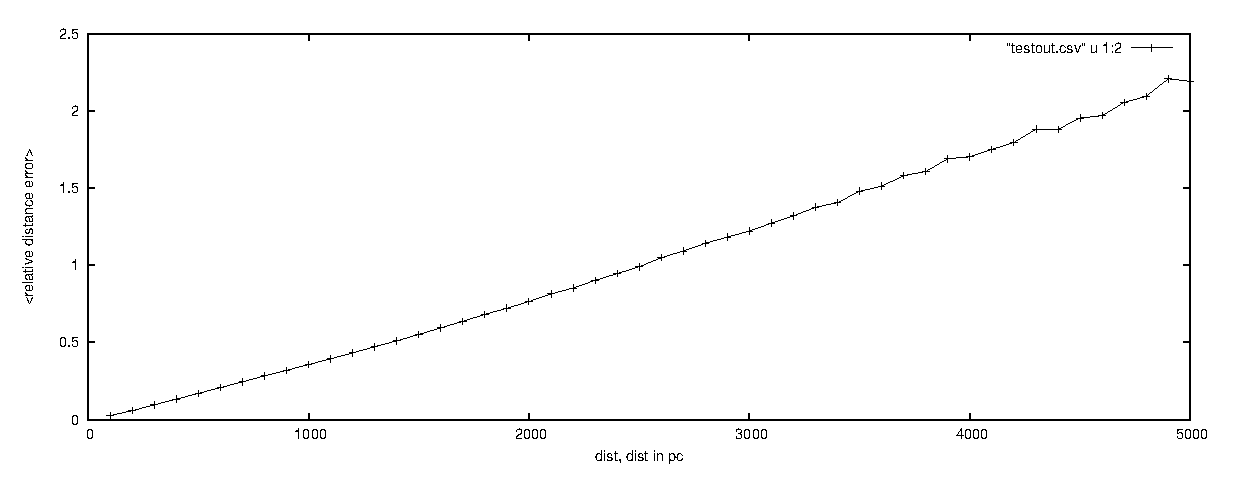
\includegraphics[width=1\linewidth,height=0.4\textheight]{distvserr.eps}\\
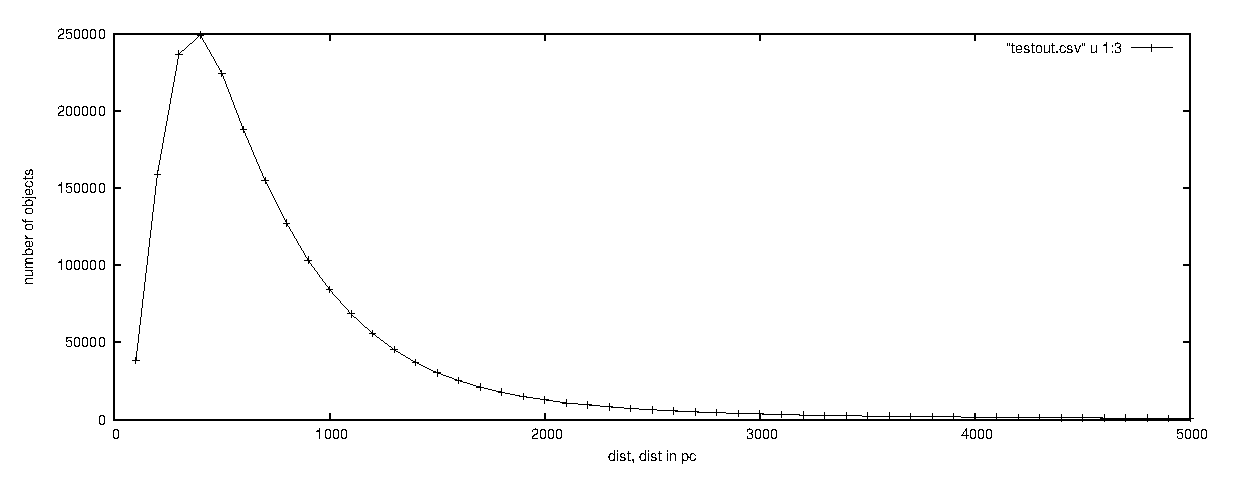
\includegraphics[width=1\linewidth,height=0.4\textheight]{distvsN.eps}
\end{frame}

\begin{frame}{TGAS: общие сведения}{Карта объектов}
\includegraphics[width=1\linewidth]{galsph.jpg}
\end{frame}

\begin{frame}{TGAS: общие сведения}{Карта средних расстояний до объектов}
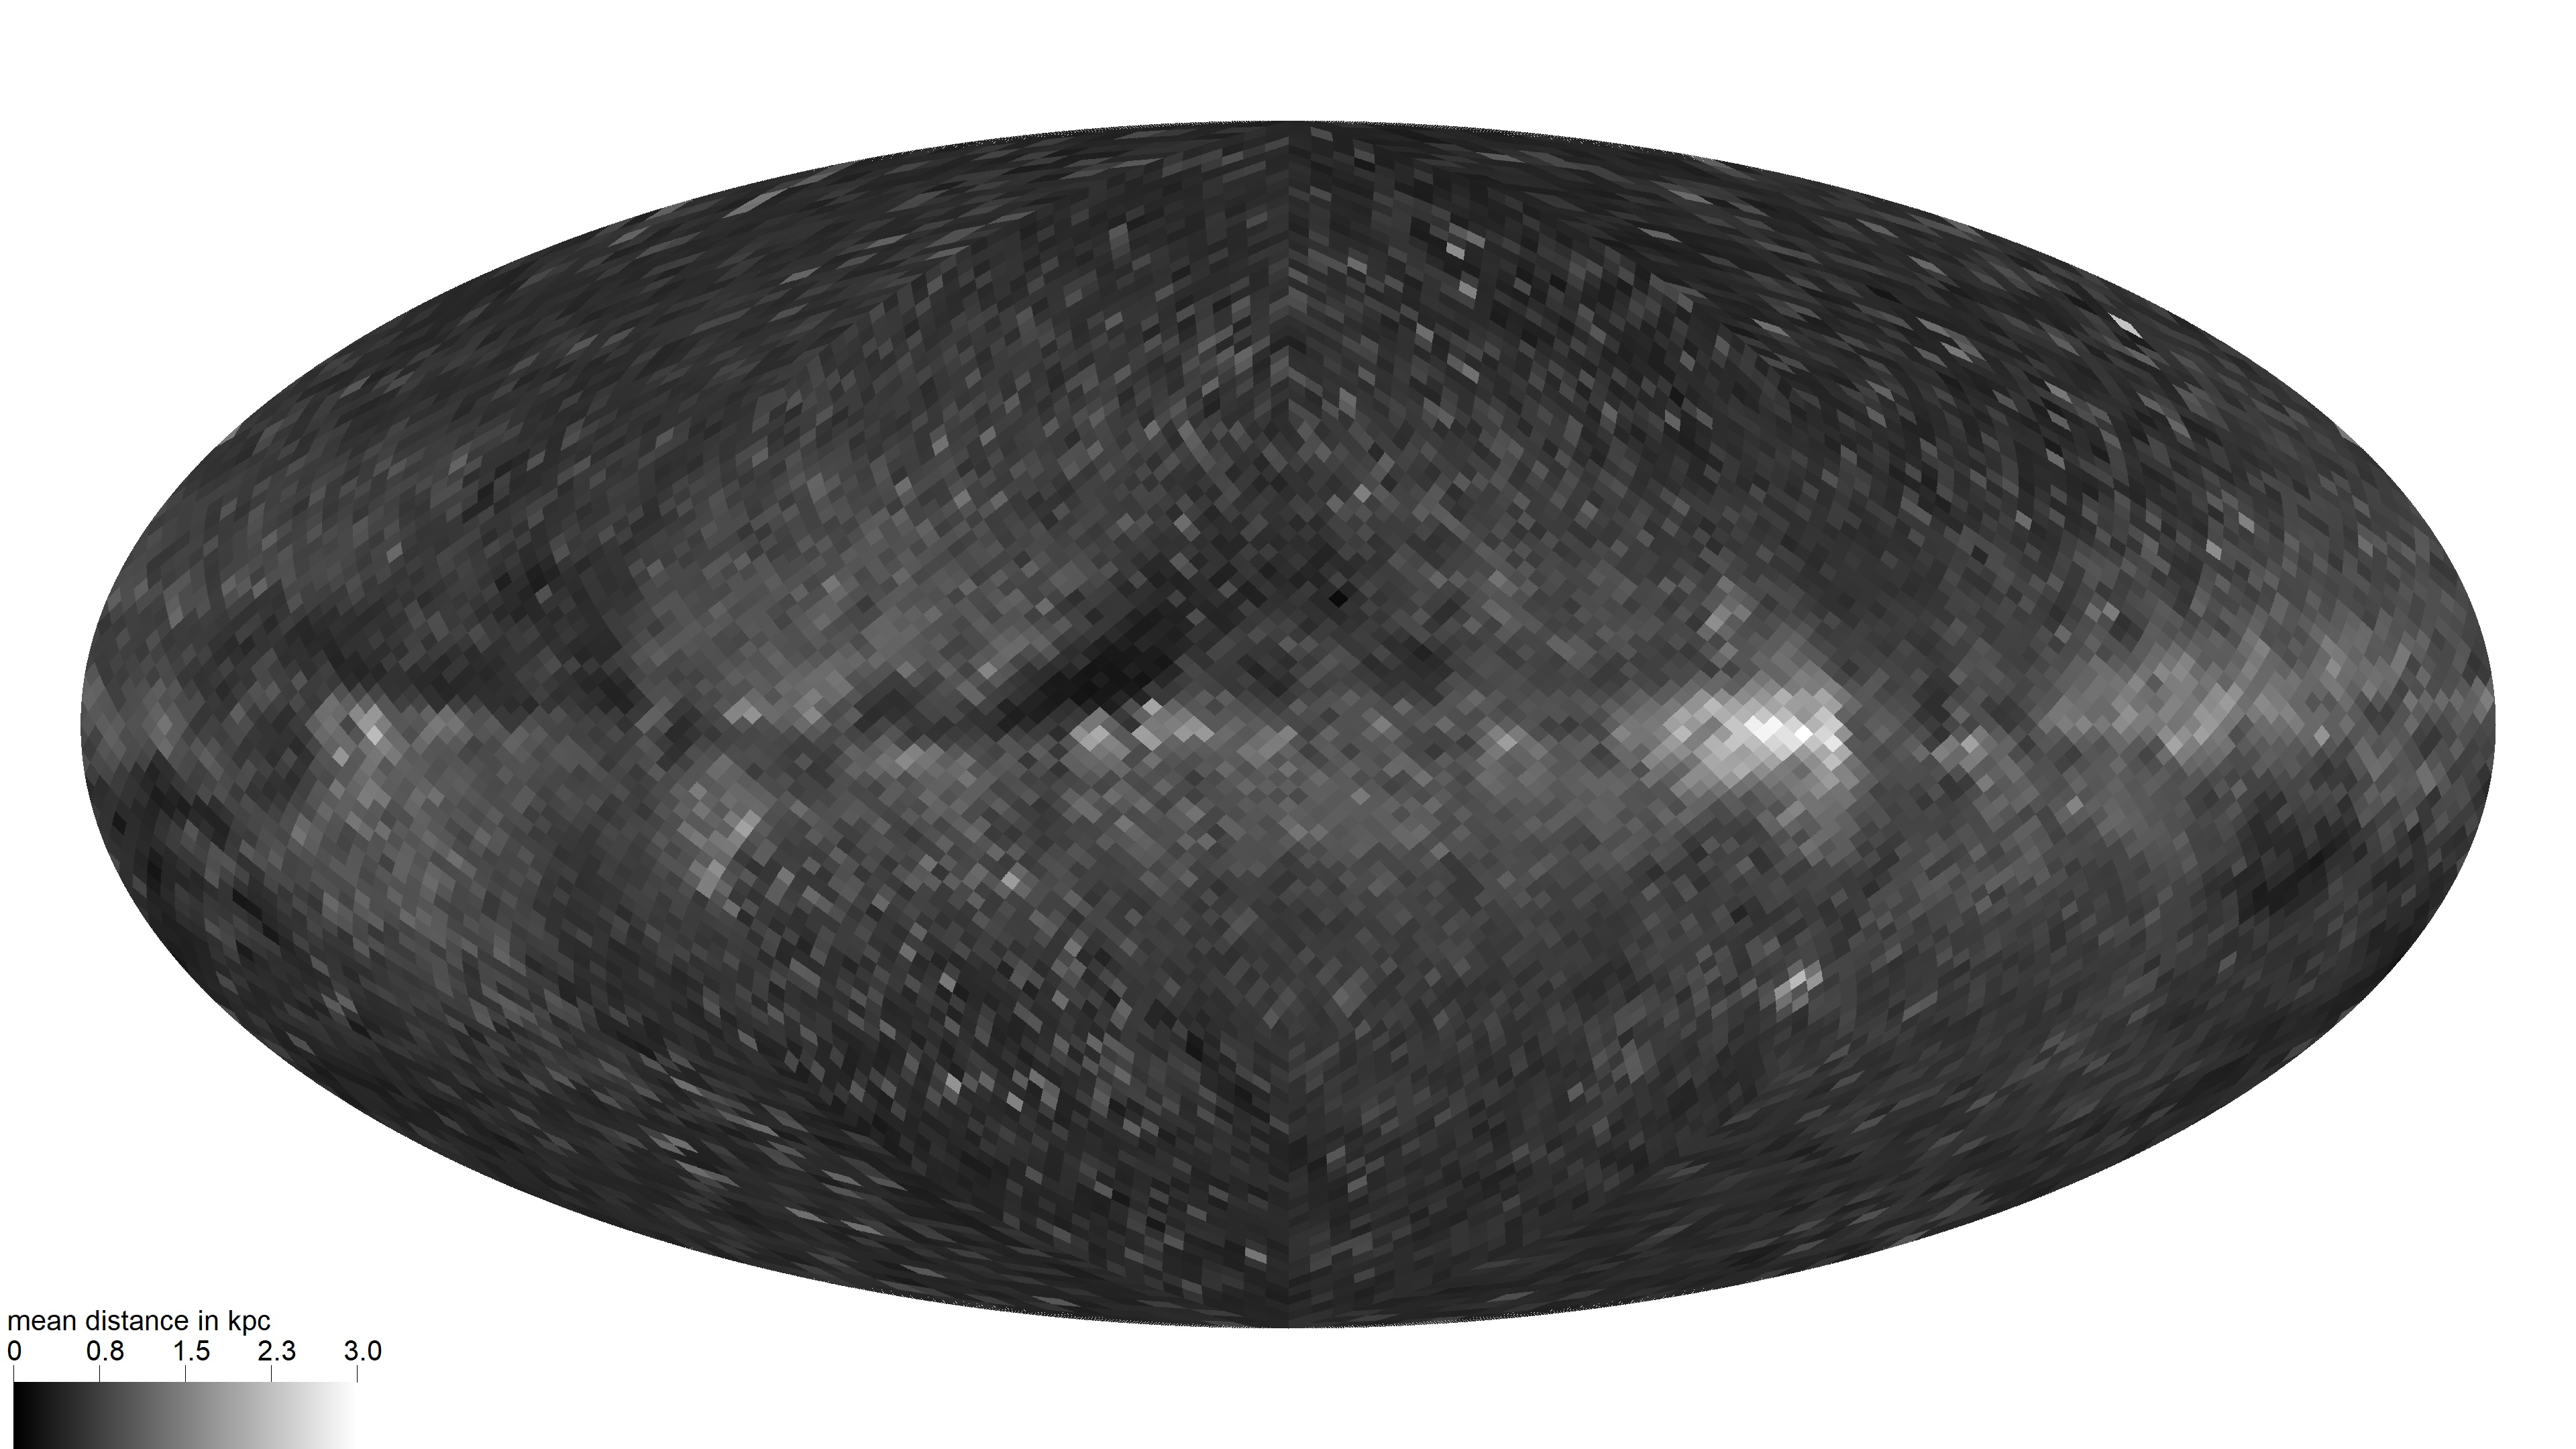
\includegraphics[width=1\linewidth]{healpdistmap.jpg}
\end{frame}
\section{Пикселизация данных на сфере}
\subsection{HEALPix}
\begin{frame}{HEALPix}{\textbf{H}ierarchical \textbf{E}qual \textbf{A}rea iso\textbf{L}atitude \textbf{Pix}elization}
\begin{itemize}
\item 12 базовых пикселей
\item Разрешение -- $N_{side}$
\item Центры пикселей одного кольца лежат на одной широте
\item Число колец $4N_{side}-1$
\item Всего пикселей $12N_{side}^2$
\end{itemize}
\end{frame}

%\begin{frame}{Формулы HEALPix}
%$p$ -- номер площадки\\
%Для северной полярной шапки ($\left|\cos\theta\right|>\frac{2}{3}$):\\
%$p_h=\frac{p+1}{2}$\\
%$1\le i<N_{side}$ -- индекс кольца\\
%$1\le j<4i$ -- индекс ячейки внутри кольца\\
%$$i=\left\lfloor\sqrt{p_h-\sqrt{\left\lfloor p_h\right\rfloor}}\right\rfloor+1$$
%$$j=p+1-2i\left(i-1\right)$$
%$$z=1-\frac{i^2}{3N_{side}^2}$$
%$$\phi=\frac{\pi}{2i}\left(j-0.5\right)$$\\
%\end{frame}

%\begin{frame}
%Для северного экваториального пояса ($\left|\cos\theta\right|<\frac{2}{3}$):\\
%$p'=p-2N_{side}\left(N_{side}-1\right)$\\
%N_{side}\le i\le 2N_{side}$\\
%1\le j\le 4N_{side}$
%$i=\left\lfloor\frac{p'}{4N_{side}}\right\rfloor + N_{side}$$
%$j=(p' \mod 4N_{side}) +1$$
%$z=\frac{4}{3}-\frac{2i}{3N_{side}}$$
%$\phi=\frac{\pi}{2N_{side}}\left(j-\frac{\left(i-N_{side}+1\right)\mod 2}{2}\right)$$
%\end{frame}

\begin{frame}{Пример пикселизации}
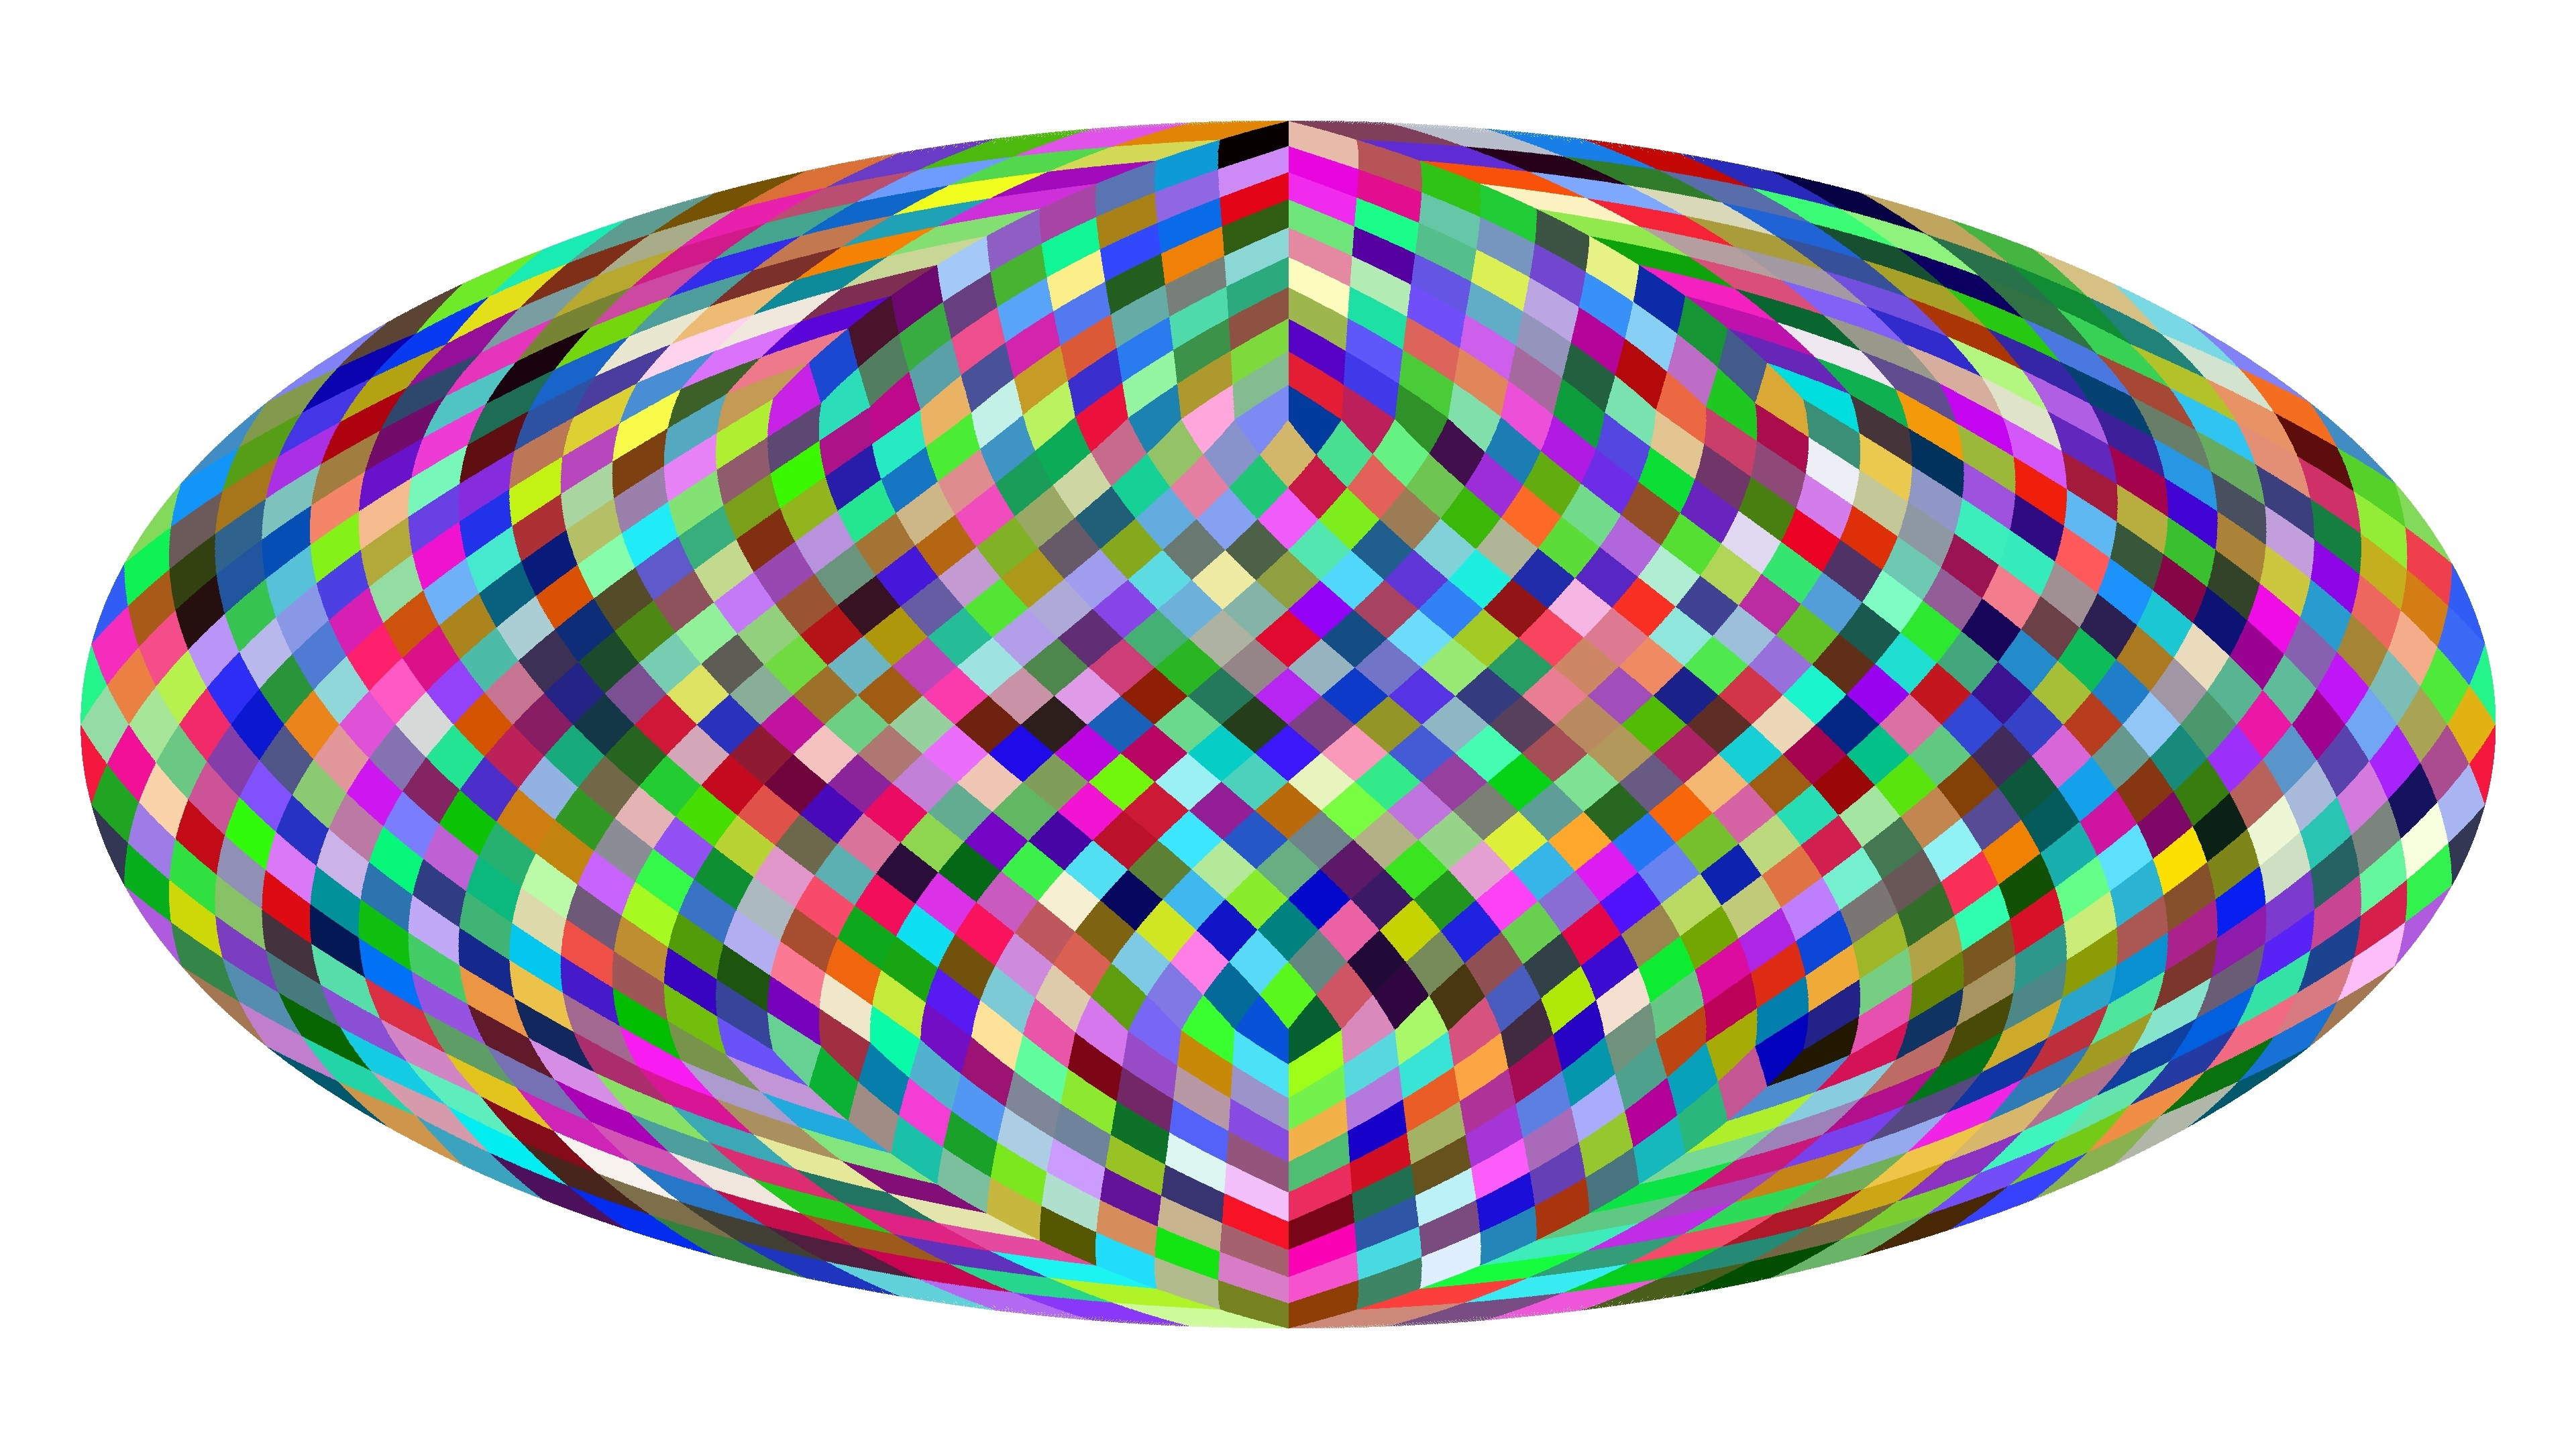
\includegraphics[width=1\linewidth]{healpexample.jpg}
\end{frame}
\subsection{Данные}

\section{Кинематические параметры}
\begin{frame}{Модель Огородникова-Милна}
\begin{equation}\label{ogorod}
V=V_0+\Omega\times r+M^+\times r
\end{equation}
$V_0$ -- скорость поступательного движения Солнца\\ $\Omega$ -- угловая скорость твердотельного вращения звездной системы \\$M^+$ -- симметричный тензор деформации поля скоростей
\end{frame}

%\begin{frame}{Описание параметров модели}
%\begin{itemize}
%\item $U$, $V$, $W$ -- компоненты вектора скорости поступательного движения Солнца ($V_0$).
%\item $\omega_1$, $\omega_2$, $\omega_3$ -- компоненты $\Omega$.
%\item $M^+_{11}$, $M^+_{22}$, $M^+_{33}$ -- параметры тензора деформации, характеризующие растяжение поля вдоль главных галактических скоростей.
%\item $M^+_{12}$, $M^+_{13}$, $M^+_{23}$ -- параметры тензора деформации, характеризующие деформацию поля в основной и двух перпендикулярных ей плоскостях.\\
%\end{itemize}
%\end{frame}

\begin{frame}{Уравнения модели}
$M_{11}^*=M_{11}^+-M_{22}^+$; $X=M_{33}^+-0.5\left(M_{11}^++M_{22}^+\right)$
\begin{multline}\label{Kmul_plus}
\mathcal{K}\mu_l\cos b=U\pi\sin l-V\pi\cos l-\omega_1\sin b\cos l-\omega_2\sin b\sin l+\\+\omega_3\cos b-M_{13}^+\sin b\sin l+M_{23}^+\sin b\cos l+M_{12}^+\cos b\cos2l-\\-\frac{1}{2}M_{11}^*\cos b\sin2l
\end{multline}
\begin{multline}\label{Kmub_plus}
\mathcal{K}\mu_b=U\pi\cos l\sin b+V\pi\sin l\sin b-W\pi\cos b+\omega_1\sin l-\\-\omega_2\cos l-\frac{1}{2}M_{12}^+\sin2b\sin2l+M_{13}^+\cos2b\cos l+M_{23}^+\cos2b\sin l-\\-\frac{1}{4}M_{11}^*\sin2b\cos2l+\frac{1}{2}X\sin2b
\end{multline}
\end{frame}

\section{Полученные результаты}
\subsection{Подготовка данных}
\begin{frame}{Выборки}
\center\begin{tabular}{|c|c|}
\hline
Расстояние, пк&Количество объектов\\
\hline
0 -- 100&38339\\
100 -- 200&159058\\
200 -- 300&236955\\
300 -- 400&249214\\
400 -- 500&224396\\
500 -- 600&187982\\
600 -- 700&155074\\
700 -- 800&127430\\
800 -- 900&103451\\
900 -- 1000&84248\\
\hline
\end{tabular}
\end{frame}

\begin{frame}{Карта плотности объектов 0--100 пк}
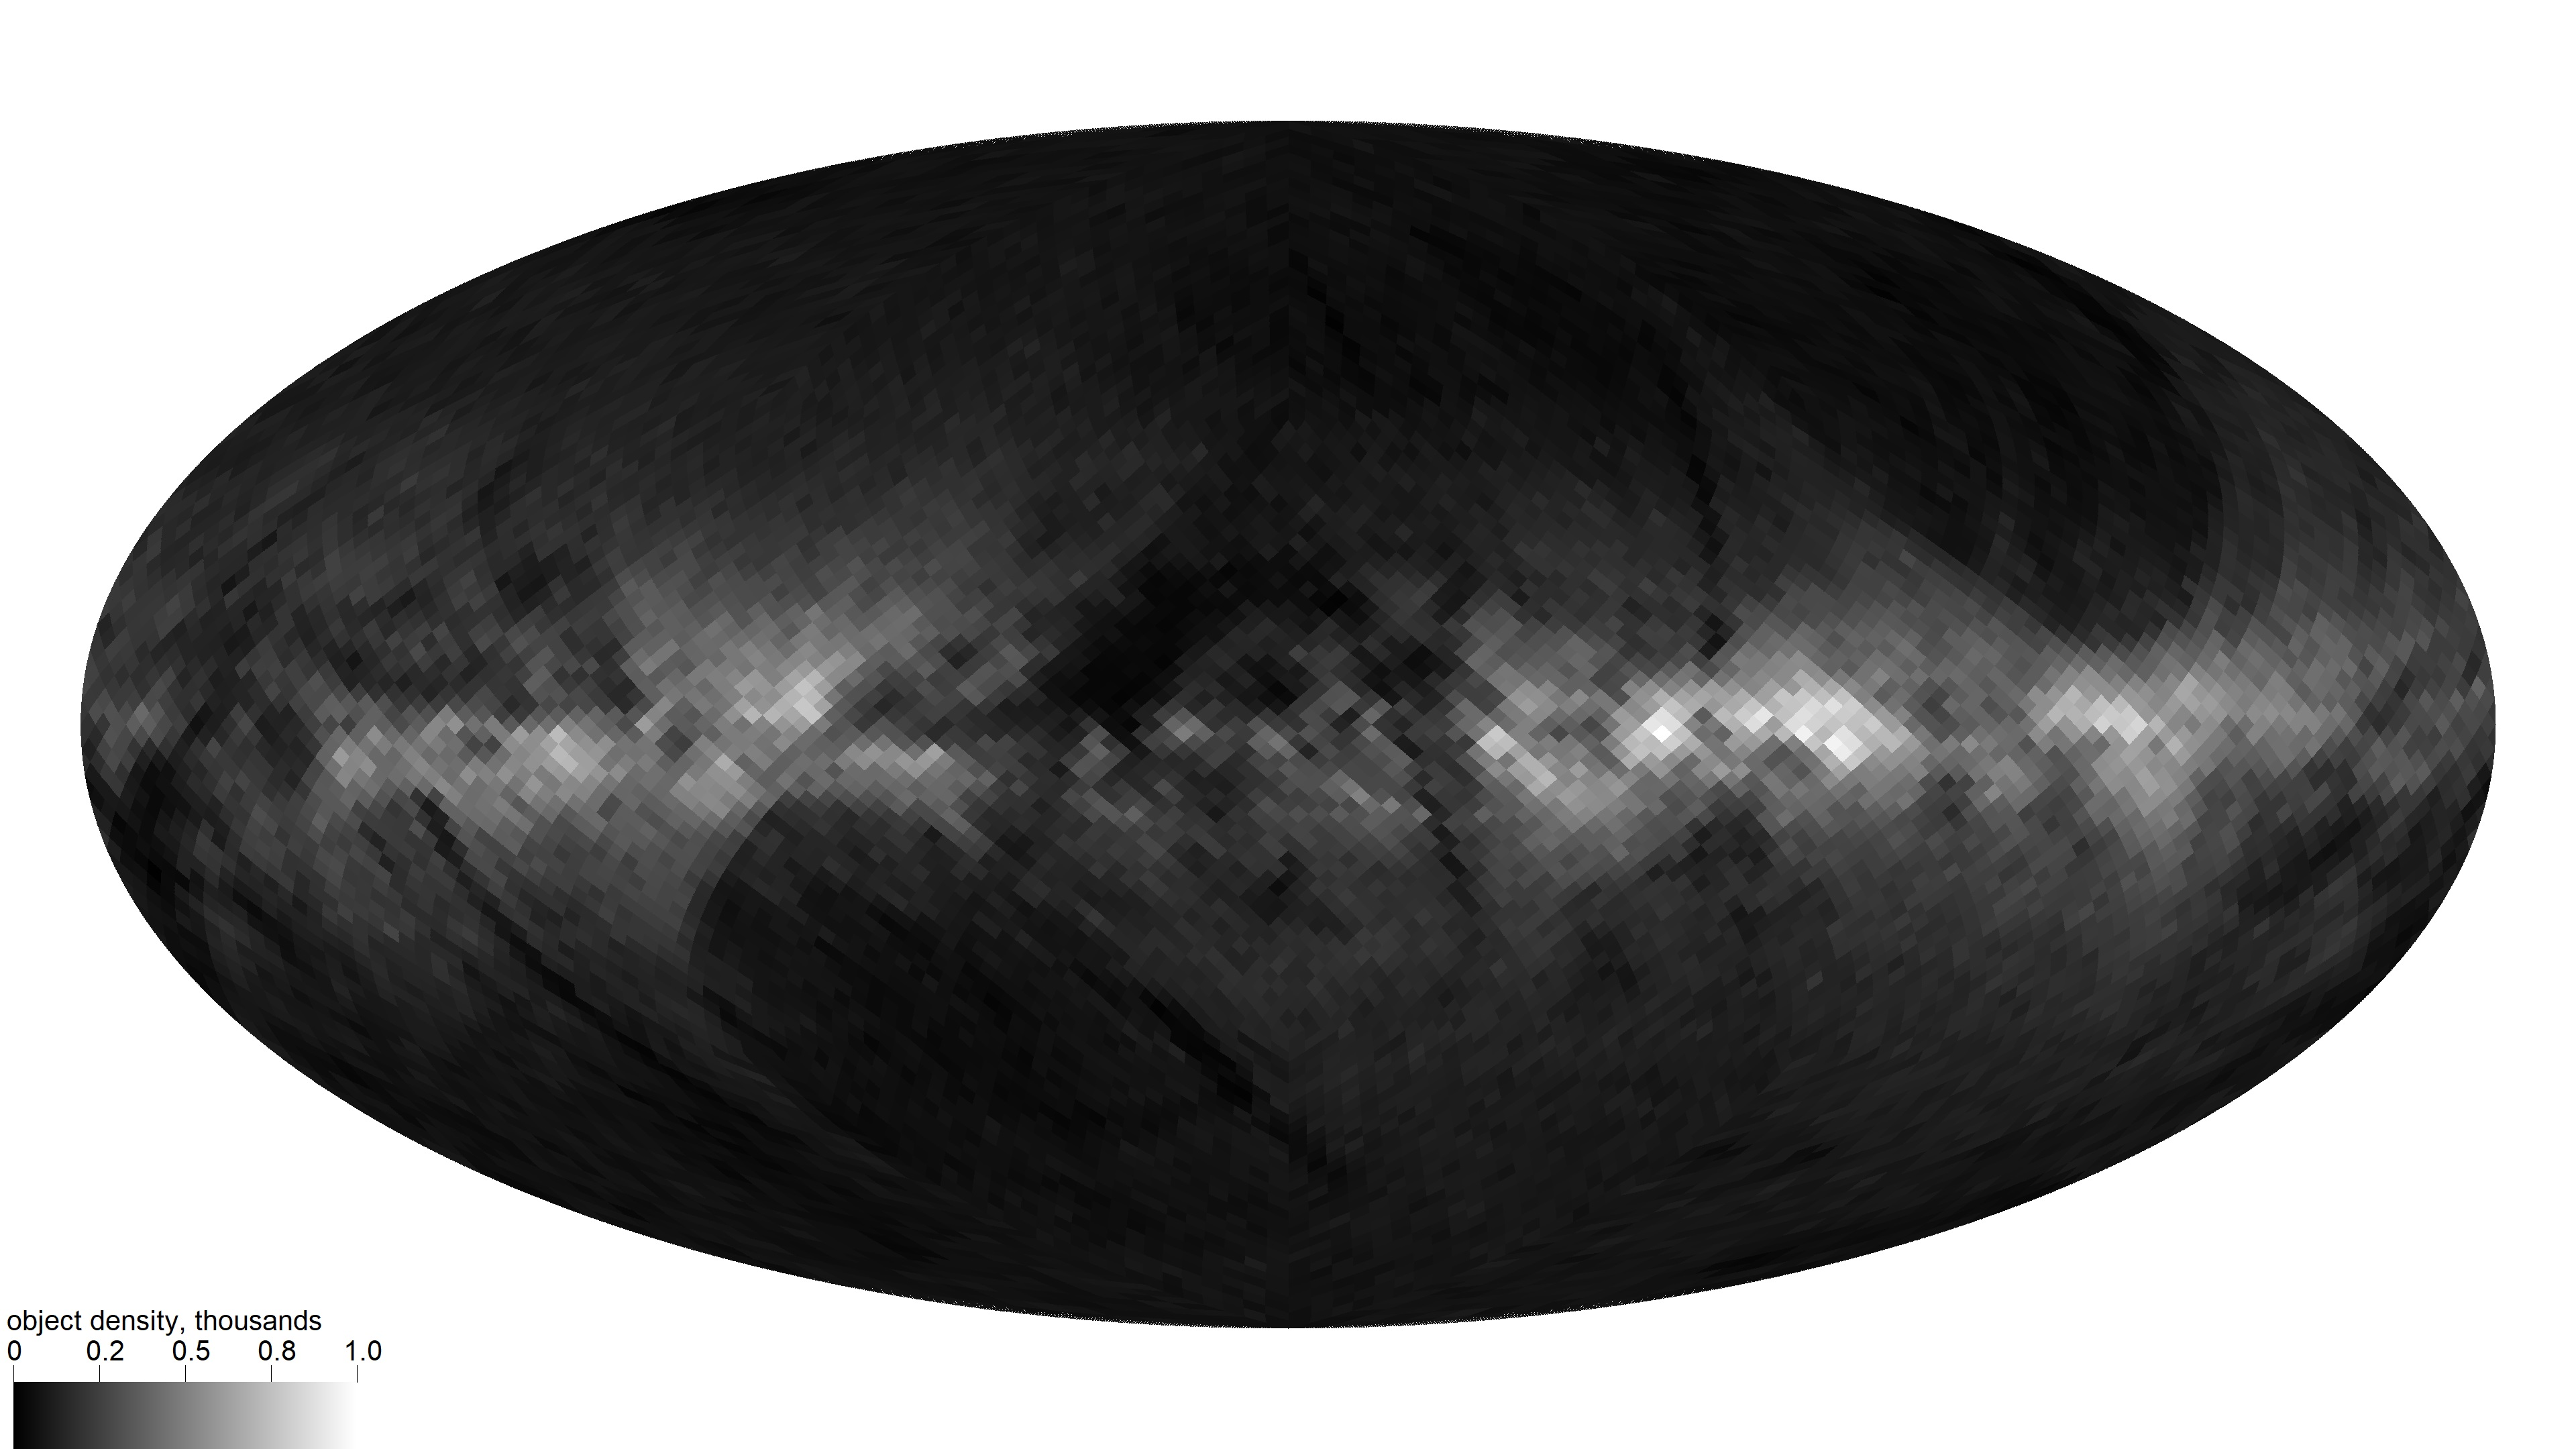
\includegraphics[width=1\linewidth]{healpdens100.jpg}
\end{frame}

\begin{frame}{Карта плотности объектов 900--1000 пк}
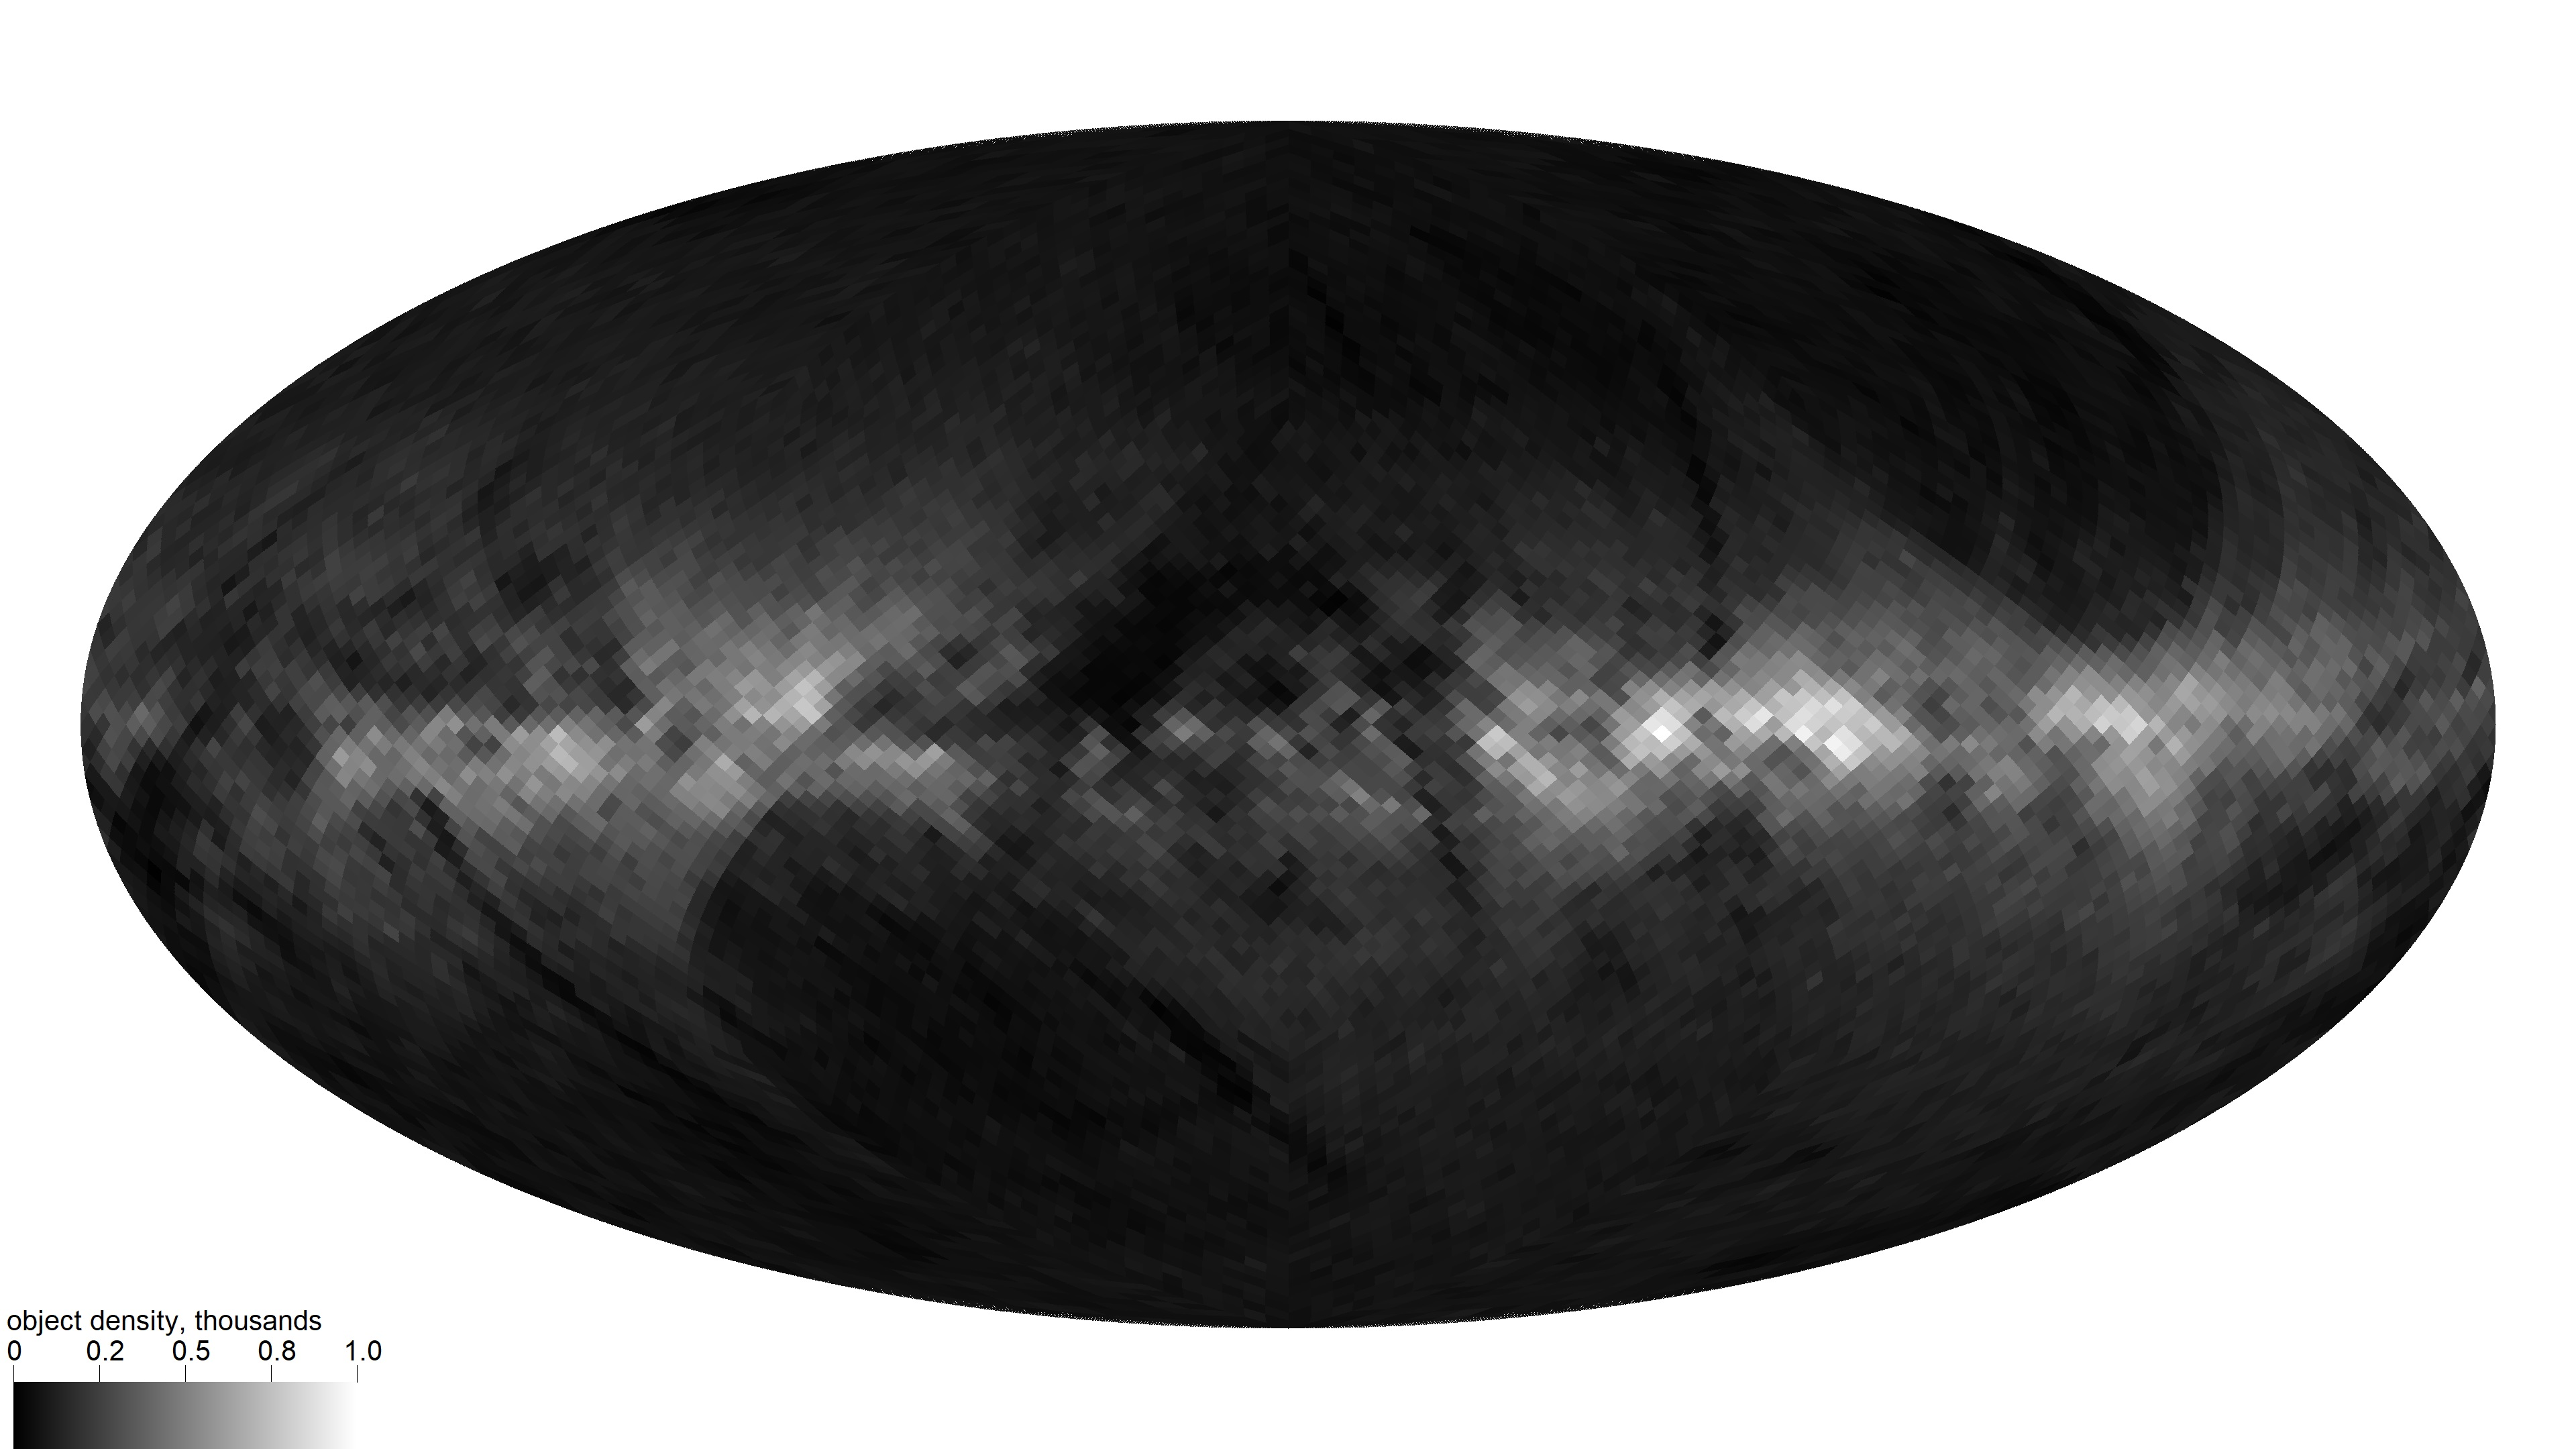
\includegraphics[width=1\linewidth]{healpdens900.jpg}
\end{frame}
\subsection{Результаты}
\begin{frame}{Результаты}{$U$, $V$, $W$}
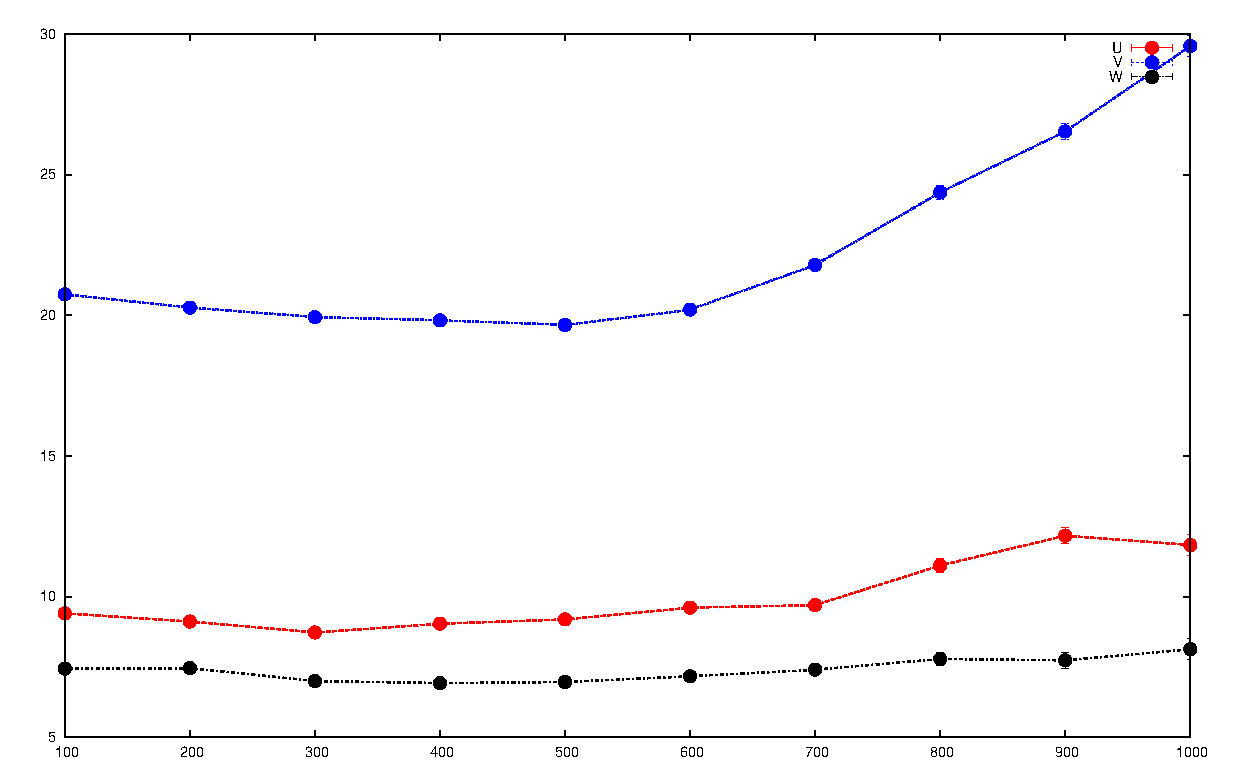
\includegraphics[width=1\linewidth]{./graphs/UVW100.eps}
\end{frame}

\begin{frame}{Результаты}{$\Omega$}
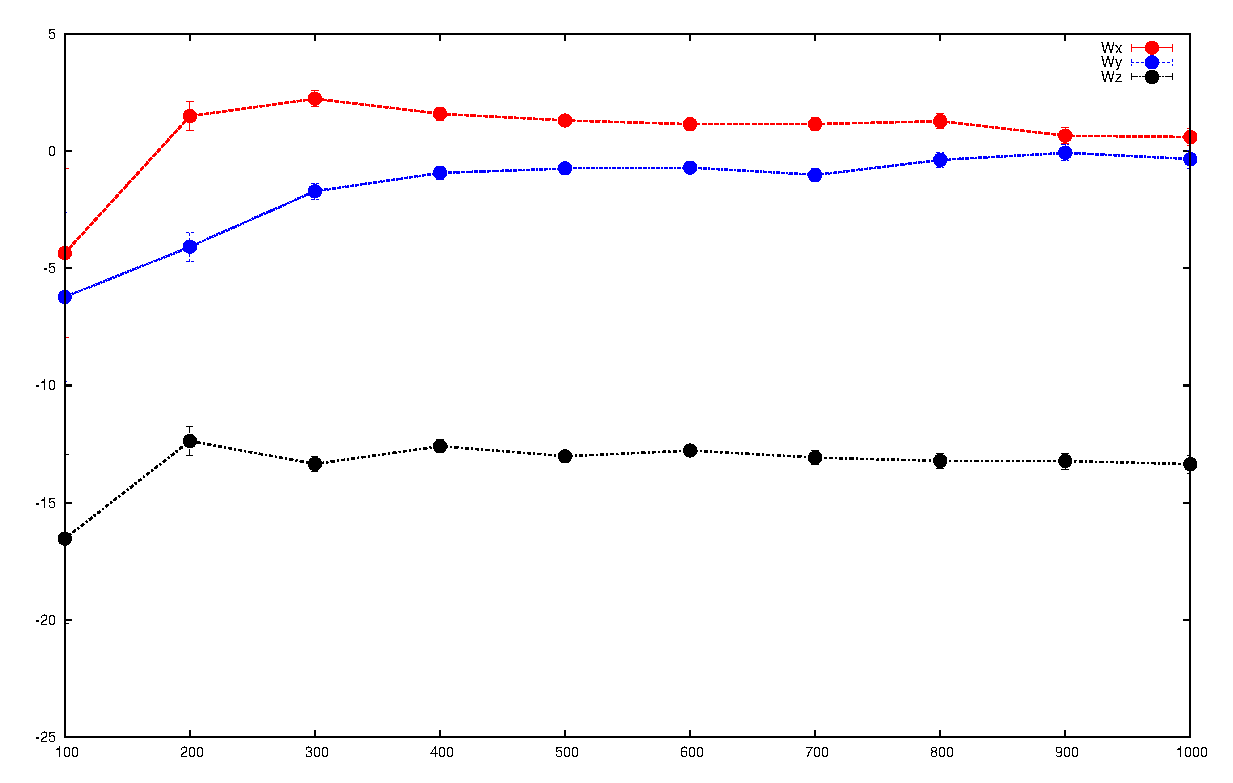
\includegraphics[width=1\linewidth]{./graphs/Omega100.eps}
\end{frame}

\begin{frame}{Результаты}{$M$}
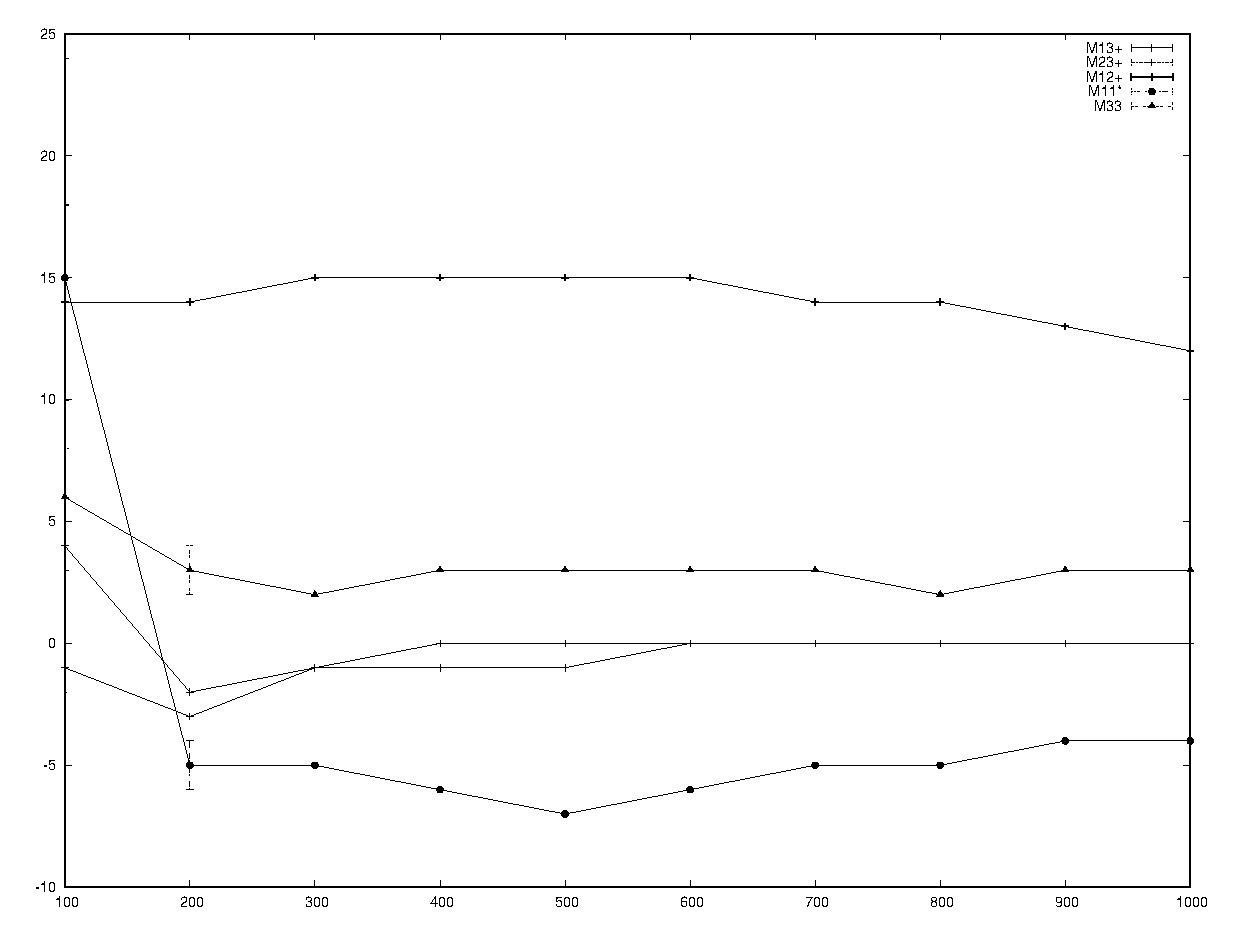
\includegraphics[width=1\linewidth]{./graphs/M100.eps}
\end{frame}

\section{Заключение}

\begin{frame}{Заключение}
\center\begin{tabular}{|c|c|c|}
\hline
Число источников&Gaia DR2&Gaia DR1\\
\hline
Общее&1692919135&1142679769\\
С пятью параметрами&1331909727&2057050\\
С двумя параметрами&361009408&1140622719\\
\hline
\end{tabular}
\end{frame}

\begin{frame}{Заключение}
\begin{itemize}
\item Параметры модели Огородникова-Милна.
\item ПО для чтения данных каталога.
\item Библиотека для визуализации данных.
\end{itemize}
\end{frame}

\begin{frame}
\center Спасибо за внимание!
\end{frame}

\begin{frame}{Джон Кеннеди}
\begin{itemize}
\item По официальной информации был убит Ли Харви Освальдом в городе Даллас 22 ноября 1963 года.
\item Мафия, в отместку за объявленный против нее крестовый поход.
\item ЦРУ, за намерения помириться с СССР.
\item Линдон Джонсон, так как Кеннеди был недоволен им на посту вице-президента.
\item Секретная служба (Джордж Хики), несчастный случай.
\item Рептилоиды.
\item Жидомасоны.
\end{itemize}
\end{frame}

\end{document}


